% \subsection{Movimento orbital relativo aplicado em missão de \gls{rvdb}}

% Ela é formulada a partir da diferença entre as posições da espaçonave perseguidora e do alvo previamente descritos no ECI, conforme apresentado na Figura~\ref{fig_movimento_relativo_LVLH}.
% Para a formulação do movimento relativo, considera-se que as posições inerciais do alvo e do perseguidor em relação ao corpo primário são $\vec r_a$ e $\vec r_p$, com $r_a=|\vec r_a|$ e $r_p=|\vec r_p|$. No problema restrito de dois corpos, a dinâmica orbital do alvo (sem aceleração de controle) é descrita por:

\subsection{Movimento orbital relativo aplicado em missão de \gls{rvdb}}

No contexto de missões de \gls{rvdb}, o movimento relativo entre o alvo e o perseguidor é formulado a partir de duas órbitas geocêntricas distintas, ambas em torno da Terra. Assim, o alvo e o perseguidor não constituem um sistema binário de corpos massivos girando em torno de um centro de massa comum. O movimento relativo de interesse é obtido pela diferença entre suas posições orbitais em relação ao mesmo corpo primário.

Sejam $\vec r_a$ e $\vec r_p$ os vetores posição inerciais do alvo e do perseguidor em relação ao centro da Terra, com $r_a=\|\vec r_a\|$ e $r_p=\|\vec r_p\|$. No problema restrito de dois corpos, a dinâmica orbital do alvo, na ausência de aceleração de controle, é descrita por:

\begin{equation}
\label{eq_movimentoalvo}
\ddot{\vec r}_a = -\frac{\mu_\oplus}{r_a^3}\,\vec r_a
\end{equation}

Enquanto a dinâmica do perseguidor (com aceleração de controle) é dada por:

% \begin{equation}
% \label{eq_movimentoperseguidor}
% \ddot{\vec r}_p
% =
% -\frac{\mu_\oplus}{r_{p}^3}\,\vec r_{p}
% +
% \frac{\vec F_{controle}}{m_{p}}.
% \end{equation}

\begin{equation}
\label{eq_movimentoperseguidor}
\ddot{\vec r}_p
=
-\frac{\mu_\oplus}{r_{p}^3}\,\vec r_{p}
+
\frac{\vec F_{controle}}{m_{p}}.
\end{equation}

O termo $\vec F_{controle}$ representa a força não gravitacional aplicada ao perseguidor, associada ao comando de controle translacional.

\begin{figure}[H]
\centering
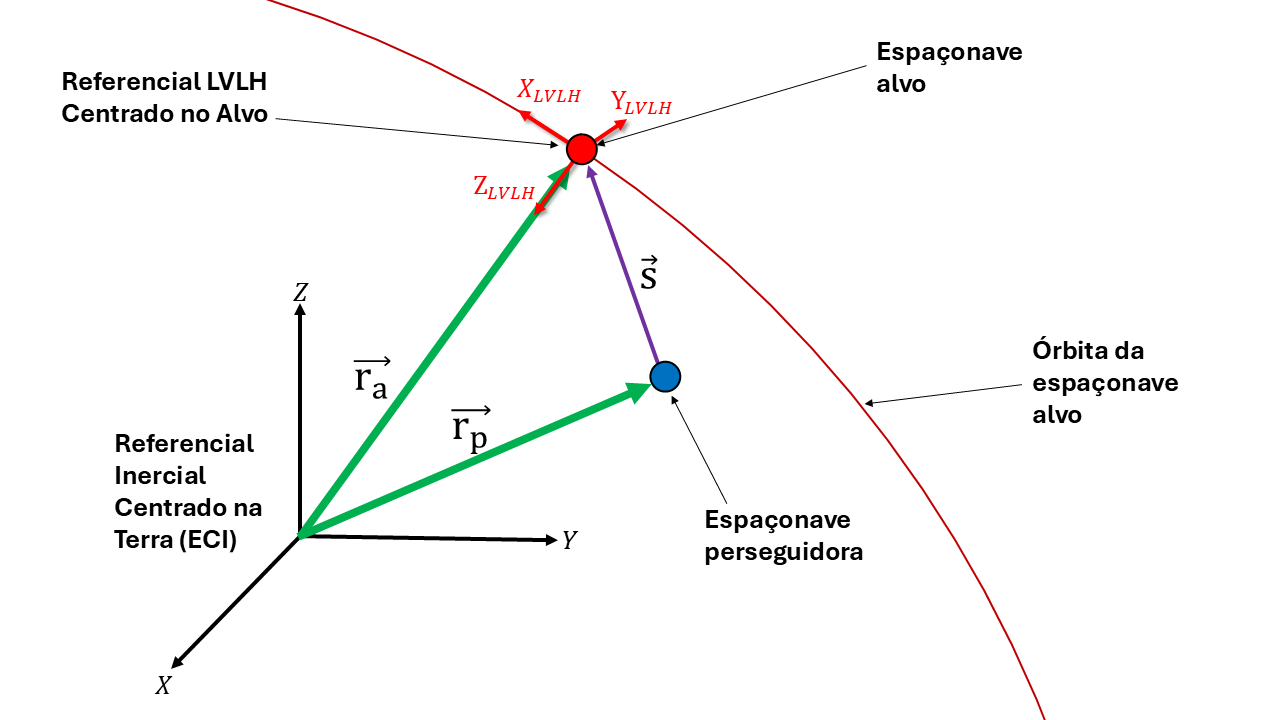
\includegraphics[width=1\linewidth]{4 Formulacao matematica/Imagens/Posicao relativa LVLH.png}
\caption{Movimento relativo das espaçonaves em relação ao referencial LVLH.}
\label{fig_movimento_relativo_LVLH}
\end{figure}

Define-se o vetor relativo $\vec{s}$, conforme apresentado na Figura~\ref{fig_movimento_relativo_LVLH}, como o vetor posição do alvo em relação ao perseguidor, isto é, orientado do perseguidor para o alvo.

\begin{equation}
\vec{r}_{p} + \vec{s} = \vec{r}_{a}.
\label{eq_soma_vetorial_triangulo}
\end{equation}

Portanto, permite isolar o vetor relativo como:

\begin{equation}
\label{eq_vetorS}
\vec{s} = \vec{r}_{a} - \vec{r}_{p}.
\end{equation}

Derivando a equação \eqref{eq_vetorS} duas vezes em relação ao tempo no referencial inercial, obtém-se a aceleração relativa:

\begin{equation}
\label{eq_vetorS_ddot}
\ddot{\vec{s}} = \ddot{\vec{r}}_{a} - \ddot{\vec{r}}_{p}.
\end{equation}

Inserindo as equações do movimento do alvo e do perseguidor na equação \eqref{eq_vetorS_ddot}, e lembrando que $\vec{s} = \vec{r}_a - \vec{r}_p$, obtém-se:

\begin{equation}
\label{eq_vetorS_ddot_substituicao}
\ddot{\vec s}
=
\left(-\mu_\oplus \frac{\vec r_a}{r_a^3}\right)
-
\left(-\mu_\oplus \frac{\vec r_{p}}{r_p^3} + \frac{\vec F_{controle}}{m_p}\right).
\end{equation}

O termo $\mu_\oplus$ é o parâmetro gravitacional do sistema. A seguir, definem-se as acelerações gravitacionais:

\begin{equation}
\label{eq_fg_rc}
\vec f_g(\vec r_p) = -\mu_\oplus \frac{\vec r_p}{r_p^3},
\end{equation}

\begin{equation}
\label{eq_fg_rt}
\vec f_g(\vec r_a) = -\mu_\oplus \frac{\vec r_a}{r_a^3}.
\end{equation}

Portanto, substituindo \eqref{eq_fg_rc} e \eqref{eq_fg_rt} em \eqref{eq_vetorS_ddot_substituicao}, a equação do movimento relativo se torna:

\begin{equation}
\label{eq_fg_rc_fg_rt}
\ddot{\vec s}
=
\vec f_g(\vec r_a) - \vec f_g(\vec r_p) - \frac{\vec F_{controle}}{m_p}.
\end{equation}

%%%%%%%%%%%%%%%%%%%%%%%%%%%%%%%%%%%

% Para simplificar a diferença entre os termos gravitacionais na equação do movimento relativo, que é suficiente para representar o posicionamento relativo entre as espaçonaves quando eles estão próximos. Considerando a diferença gravitacional obtida na equação do movimento, a linearização resulta em:
Para simplificar a diferença entre os termos gravitacionais na equação do movimento relativo, lineariza-se o campo gravitacional em torno da posição do alvo, assumindo que a distância relativa entre as espaçonaves é pequena em comparação com o raio orbital. Nessas condições, a diferença gravitacional pode ser aproximada por uma expansão de primeira ordem, resultando em:

\begin{equation}
\label{eq_linearizandoJacobiana}
\vec f_g(\vec r_{a}) - \vec f_g(\vec r_{p}) \approx \mathbf{J}(\vec r_{a})\,\vec s.
\end{equation}

O vetor $\vec s$, conforme definido anteriormente, é dado pela Equação~\ref{eq_vetorS}.
A matriz $\mathbf{J}(\vec r_a)$ é a Jacobiana do campo gravitacional avaliada na posição do alvo, definida como:

\begin{equation}
\mathbf{J}(\vec r_a) \;\triangleq\; \left.\frac{\partial \vec f_g}{\partial \vec r}\right|_{\vec r=\vec r_a}.
\end{equation}

Essa matriz de derivadas parciais fornece a inclinação local do campo gravitacional, permitindo aproximar a variação da força através da relação linear com o deslocamento $\vec{s}$ \cite{khalil2002nonlinear}.
Aplicando essa definição ao campo gravitacional newtoniano $\vec f_g(\vec r)=-\mu_\oplus\,\vec r/r^{3}$, os elementos da diagonal principal da matriz $\mathbf{J}$ são obtidos por \cite{fehse2003}:

\begin{equation}
\label{eq_jacobianaDiagonal}
J_{ii} \;=\;
\frac{\partial f_{g,i}}{\partial r_i} \;=\;
-\frac{\mu}{r_a^3}\!\left(1 - 3\,\frac{r_{a,i}^2}{r_a^2}\right), \quad (i=1,2,3).
\end{equation}

Sendo que $r_{a,i}$ representa a $i$-ésima componente do vetor posição do alvo e $r_a$ é o seu módulo.
Os termos fora da diagonal principal da matriz Jacobiana são dados por \cite{fehse2003}:

\begin{equation}
\label{eq_jacobianaForaDiagonal}
J_{ij} =
\frac{\partial f_{g,i}}{\partial r_j} =
3 \frac{\mu}{r_a^3} \frac{r_i r_j}{r_a^2}, \quad (i \neq j).
\end{equation}

O termo $r_i$ e $r_j$ são as componentes do vetor posição do alvo $\vec{r}_a$.
Agrupando os termos diagonais e fora da diagonal, a matriz Jacobiana $\mathbf{J}(\vec{r}_a)$ completa é definida como:

\begin{equation}
\label{eq_jacobianaGenerica}
\mathbf{J}(\vec{r}_a) = -\frac{\mu}{r_a^3}
\begin{bmatrix}
1 - 3\frac{r_x^2}{r_a^2} &  -3\frac{r_x r_y}{r_a^2} &  -3\frac{r_x r_z}{r_a^2} \\
-3\frac{r_y r_x}{r_a^2} & 1 - 3\frac{r_y^2}{r_a^2} & -3\frac{r_y r_z}{r_a^2} \\
-3\frac{r_z r_x}{r_a^2} & -3\frac{r_z r_y}{r_a^2} & 1 - 3\frac{r_z^2}{r_a^2}
\end{bmatrix}.
\end{equation}

Dessa forma, a linearização da diferença das forças gravitacionais, apresentada em \eqref{eq_linearizandoJacobiana}, pode ser escrita como:

\begin{equation}
\label{eq_linearizandoJacobiana2}
\vec f_g(\vec r_{a}) - \vec f_g(\vec r_{p}) \approx \mathbf{J}(\vec{r}_a)\,\vec s.
\end{equation}

Substituindo \eqref{eq_linearizandoJacobiana2} na equação do movimento relativo \eqref{eq_fg_rc_fg_rt}, obtém-se a equação dinâmica linearizada para o vetor $\vec{s}$:

\begin{equation}
\label{eq_fg_rc_fg_rt_linearizada}  
\ddot{\vec{s}} = \mathbf{J}(\vec{r}_a)\,\vec{s} - \frac{\vec F_{controle}}{m_{p}}.
\end{equation}

%%%%%%%%%%%%%%%%%%%%%%%%%%%%%%%%%%%%%%%

Para expressar a dinâmica relativa no referencial orbital \gls{lvlh}, aplica-se o Teorema do Transporte, que relaciona as derivadas temporais de um vetor observadas em referenciais com movimento relativo \cite{wie2008space, symon1979}. Neste caso, o referencial \gls{lvlh} é um referencial rotativo associado à órbita do alvo.

Embora o vetor geométrico $\vec{s}$ represente o mesmo deslocamento relativo, suas derivadas temporais diferem quando observadas no referencial inercial e no referencial orbital rotativo. Denotando por $\ddot{\vec{s}}$ a derivada temporal no referencial inercial e por $\ddot{\vec{s}}^{\,*}$ a derivada temporal no referencial \gls{lvlh}, a relação cinemática completa é dada por:

\begin{equation}
\label{eq_TransporteSymon1979}
\ddot{\vec s} = 
\ddot{\vec s}^{\,*}
+ 2 \vec{\omega} \times \dot{\vec s}^{\,*}
+ \vec{\omega} \times (\vec \omega \times \vec {s})
+ \dot{\vec{\omega}} \times \vec{s}.
\end{equation}

Os termos $\vec{\omega}$ e $\dot{\vec{\omega}}$ representam, respectivamente, a velocidade angular e a aceleração angular do referencial \gls{lvlh} em relação ao referencial inercial.
Igualando a relação cinemática dada por \eqref{eq_TransporteSymon1979} à equação dinâmica linearizada \eqref{eq_fg_rc_fg_rt_linearizada}, obtém-se a equação do movimento relativo no referencial \gls{lvlh} \cite{fehse2003}:

\begin{equation}
\label{eq_relativo_LVLHgeral}
\ddot{\vec s}^{\,*}
+ 2 \vec \omega \times \dot{\vec s}^{\,*} 
+ \vec \omega \times (\vec \omega \times \vec{s})
+ \dot{\vec \omega} \times \vec{s}
- \mathbf{J}(\vec r_a)\,\vec{s}
= - \frac{\vec{F}_p}{m_p}.
\end{equation}

A Equação~\eqref{eq_relativo_LVLHgeral} representa a dinâmica relativa linearizada no referencial \gls{lvlh}, ainda em sua forma vetorial geral.
Para o caso particular em que a órbita do alvo é circular, a velocidade angular do referencial \gls{lvlh} tem módulo constante e, portanto, $\dot{\vec{\omega}}=\vec{0}$. Além disso, ao alinhar os eixos do referencial \gls{lvlh} com a geometria orbital do alvo, a Equação~\eqref{eq_relativo_LVLHgeral} pode ser reescrita em forma escalar, resultando nas equações de Hill, também conhecidas como equações de Clohessy--Wiltshire, apresentadas a seguir.